\documentclass[10pt]{article}
\usepackage{extsizes}
\usepackage[affil-it]{authblk}
\usepackage[T1]{fontenc}
\usepackage[utf8]{inputenc}
\usepackage[english]{babel}
\usepackage{amsfonts}
\usepackage{amsmath}
\usepackage{amsthm}
\newtheorem{thm}{Theorem}
\usepackage{graphicx}
\usepackage{subfigure}
\usepackage{enumitem}
\usepackage{amssymb}
\usepackage{cancel}
\usepackage{hyperref}
\usepackage{listings}
\usepackage{color}

\usepackage[explicit]{titlesec}
\usepackage{xkeyval}
\usepackage{tikz}
\usetikzlibrary{tikzmark,calc}
\usepackage{lipsum}

\newlength\LeftSep
\newlength\RightSep
\newlength\TitleWd
\newlength\VertLineWd
\newlength\SpaceBefore
\newlength\SpaceAfter
\newlength\RuleAddition
\newcommand\SectionFont{\normalfont\Large\bfseries}
\newsavebox\TitleBox
\newcounter{tmp}

\setlength\LeftSep{\marginparsep}
\setlength\RightSep{\marginparsep}
\setlength\TitleWd{0.6666\textwidth}
\setlength\VertLineWd{1pt}
\setlength\SpaceBefore{3.5ex plus 1ex minus .2ex}
\setlength\SpaceAfter{2.3ex plus .2ex}
\setlength\RuleAddition{0pt}

\makeatletter
\define@key{fctaylor}{leftsep}{\setlength\LeftSep{#1}}
\define@key{fctaylor}{rightsep}{\setlength\RightSep{#1}}
\define@key{fctaylor}{titlewidth}{\setlength\TitleWd{#1}}
\define@key{fctaylor}{verticalrulewidth}{\setlength\VertLineWd{#1}}
\define@key{fctaylor}{spacebefore}{\setlength\SpaceBefore{#1}}
\define@key{fctaylor}{spaceafter}{\setlength\SpaceAfter{#1}}
\define@key{fctaylor}{sectionfont}{\renewcommand\SectionFont{#1}}
\define@key{fctaylor}{ruleaddition}{\setlength\RuleAddition{#1}}

\newcommand\FCsectionformat[1][]{%
\setkeys{fctaylor}{#1}
\titleformat{\section}
  {\SectionFont}{}{0em}
  {%
    \parbox[t]{1em}{\thesection}\hspace{\LeftSep}%
    \stepcounter{tmp}%
    \tikz[remember picture]
      \draw[overlay,line width=\VertLineWd] 
        ([xshift=-\RightSep,yshift=\dimexpr\ht\strutbox+\RuleAddition\relax]pic cs:start-\thetmp) -- 
        ( $ ({pic cs:start-\thetmp}|-{pic cs:end-\thetmp}) + (-\RightSep,\dimexpr+\ht\strutbox-\baselineskip-\RuleAddition\relax)$ );%
    \hspace{\RightSep}% 
    \parbox[t]{\TitleWd}{%
      \SectionFont\raggedright\strut%
      \tikzmark{start-\thetmp}##1\tikzmark{end-\thetmp}\strut}%
  }
\titleformat{name=\section,numberless}
  {\SectionFont}{}{0em}
  {%
   \hspace*{\dimexpr1em+\LeftSep\relax}%
    \stepcounter{tmp}%
    \tikz[remember picture]
      \draw[overlay,line width=\VertLineWd] 
        ([xshift=-\RightSep,yshift=\dimexpr\ht\strutbox+\RuleAddition\relax]pic cs:start-\thetmp) -- 
        ( $ ({pic cs:start-\thetmp}|-{pic cs:end-\thetmp}) + (-\RightSep,\dimexpr+\ht\strutbox-\baselineskip-\RuleAddition\relax)$ );%
    \hspace{\RightSep}% 
    \parbox[t]{\TitleWd}{%
      \SectionFont\raggedright\strut%
      \tikzmark{start-\thetmp}##1\tikzmark{end-\thetmp}\strut}%
   }
}
\titlespacing*{\section}
  {0pt}{\SpaceBefore}{\SpaceAfter}
\titlespacing*{name=\section,numberless}
  {0pt}{\SpaceBefore}{\SpaceAfter}
\makeatother

\FCsectionformat

\usepackage{titling}


\title{The Role of Machine Learning and Neural Networks Across the Decades}
\date{}
\author{Paolo Didier Alfano}
\affil{Università degli Studi di Torino}

\begin{document}
\maketitle
\begin{abstract}
Artificial intelligence and machine learning based on neural networks have seen an ever-increasing diffusion in recent years. In this short essay, we will illustrate the birth and development of artificial neural networks by analyzing three vitally important papers on the subject. As we will see, these papers provide a fundamental contribution to computer science, not only in the field of artificial neural networks.
\end{abstract}
\section{Introduction}
In recent years, neural networks, particularly thanks to the developments in deep learning techniques, have been attracting much attention. To realize this fact, it is enough to type the words \emph{artificial neural network} into any search engine. In the news section, it will be possible to find articles from the world's most important newspapers of recent publication. It would be difficult to find a field of study to which the term \emph{pervasive} can be applied as effectively. Recently, we have seen neural network-based algorithms perform activities considered achievable exclusively by humans: driving vehicles, painting, writing poems. These exceptional developments are partly the result of increased computational power, but are primarily the consequence of surprisingly ancient solid theoretical foundations. In the following, we will see how the context in which neural networks are born and develop has had a strong impact on the research and studies conducted. The path we will follow consists of three parts:
\begin{enumerate}
	\item In the first part, we will study the origins of neural networks. We will see, thanks to the article by \href{https://en.wikipedia.org/wiki/Warren_Sturgis_McCulloch}{Warren McCulloch} and \href{https://en.wikipedia.org/wiki/Walter_Pitts}{Walter Pitts}, the first study on artificial neural networks.
	\item Next, we will look at the study that lays a theoretical foundation for neural networks, by \href{https://en.wikipedia.org/wiki/Stephen_Cole_Kleene}{Stephen Kleene}.
	\item Finally, we will see how, in an already mature context, the concept of the modern neural network based on automata was developed. For this last part, we will refer to a work by \href{https://en.wikipedia.org/wiki/Marvin_Minsky}{Marvin Minsky}.
\end{enumerate}

\section{The Origins: McCulloch and Pitts}\label{ch: origins}
The history of neural networks begins when \href{https://en.wikipedia.org/wiki/Warren_Sturgis_McCulloch}{Warren McCulloch} meets \href{https://en.wikipedia.org/wiki/Walter_Pitts}{Walter Pitts}. Their first meeting dates back to 1942, in Chicago. These two personalities remained connected until their respective deaths, both occurring in 1969, a few months apart from each other.\footnote{In particular, the life of Walter Pitts, rich in notable events, would deserve a separate essay. For completeness, we report \href{http://nautil.us/issue/21/information/the-man-who-tried-to-redeem-the-world-with-logic}{an article} that accurately describes Pitts' life, starting from his correspondence with McCulloch.}\
In 1943, thanks to McCulloch's interest in the propagation of electrical signals in the cerebral cortex and Walter Pitts' early talent in logical-mathematical studies, the paper theorizing artificial neural networks for the first time was published\cite{McCulloch1943}.\\
The purpose of the paper is clear from the summary: due to the \emph{all-or-none} nature of nerve activity, it can be represented using propositional logic.\\
Initially, some fundamental information regarding the biological neuron is provided: structure, propagation of the electrical signal, and particularly the concept of \emph{state}.\\
Indeed, a neuron can be, at any given moment in time, either \emph{excited} or \emph{at rest}. The intuitive idea is that a neuron changes its state from "at rest" to "excited" if it receives a sufficient number of electrical stimuli from neighboring neurons. This number is called the \emph{threshold value}. After a few milliseconds in an excited state, during which it may produce an electrical signal, the neuron returns to its resting state.\\
Connecting multiple neurons together, we obtain a \emph{neural network}.\\
As we mentioned, when a neuron is excited, it can emit a signal. Neuronal signals are of two types:
\begin{itemize}
	\item Excitatory: sent to another neuron, they contribute to reaching the threshold value of the recipient.
	\item Inhibitory: sent to another neuron, they prevent it from transitioning from the resting state to the excited state.
\end{itemize}
The introductory part concludes by analyzing a problem: a signal propagating from one end of the neural network to the other is destined to extinguish once it has traversed it. The solution to this problem is to introduce cycles that allow the signal to persist over time within the network. Therefore, the paper by McCulloch and Pitts first studies networks without cycles. In the last part, it deals with cyclic networks.\\
In this regard, the article introduces the concept of \emph{order}: in a network, the order is the number of neurons to remove to make it acyclic. We note, in particular, that zero-order networks are already cycle-free.\\
Immediately after, artificial neural networks are introduced with some assumptions: neuron activity is Boolean; to excite a neuron, a certain number of excitatory signals are needed simultaneously; a single inhibitory signal to a neuron prevents its excitation; the structure does not change over time.\\
The mathematical representation of McCulloch and Pitts is based on the symbolism of Carnap\cite{Carnap1937} and Russell\cite{Russell1925}. As also noted by Stephen Kleene, this notation is less readable than that used in subsequent articles.\\
The $m$ neurons belonging to a certain network $\mathcal{N}$ are represented using the notation
\begin{center}
	$c_1,\ \ldots\ , c_m$
\end{center}
In particular, the neurons are divided into two groups:
\begin{itemize}
	\item \emph{Peripheral afferents}: the neurons that do not receive input from other neurons; they are the ones from which the initial signal propagates. We assume that the signal activating the peripheral afferents comes from the outside.
	\item All other neurons. Kleene refers to these neurons as \emph{inner neurons}. They are excited over time thanks to the propagation of the signal produced by the peripheral afferents.
\end{itemize}
Furthermore, the notation $N_i(t)$ indicates that neuron $i$ is excited at time $t$. With $N_i$, we indicate the actions of neuron $i$ over time.\\
The concept of \emph{solution} is then introduced. A solution is a set of logical sentences of the following form: "neuron $n$ is excited at a certain time $z_1$ if and only if the logical combination of inputs along with the signal propagation over time allows its excitation." We report a generic logical sentence $S_i$ belonging to the set of solutions:
\begin{equation}
	S_i: N_{p+1}(z_1) \equiv Pr_i(N_1, N_2, \ldots, N_p, z_1)
\end{equation}
Where $z_1$ is the time, $Pr_i$ is the $i$-th predicate belonging to the set of solutions, and $N_1, \ldots, N_p$ are the peripheral afferents of the neural network.\\

Through the concepts just seen, the article introduces a new class of logical expressions called \emph{temporal propositional expressions} or \emph{TPE}. The propositions belonging to this logic have a single free variable identifiable with discrete time and are recursively defined as follows:
\begin{enumerate}
	\item Every predicate with a single argument is a TPE.
	\item The operations of disjunction $\vee$, conjunction $\wedge$, and negation $\neg$ between TPEs produce a TPE. Furthermore, a TPE in which we appropriately replace the temporal value with its predecessors generates a TPE.
	\item Nothing else is a TPE.
\end{enumerate}
After introducing TPEs, McCulloch and Pitts proceed to prove the most important theorem about acyclic networks:
\begin{thm}
	Every TPE can be implemented by a zero-order network.
\end{thm}
This allows us to assert that given a logical expression, it is always possible to represent it using a cycle-free neural network.\
Later, the article presents six additional theorems on acyclic networks. For example, they prove the complement of the theorem just stated: "given a zero-order network, such network can be solved by a TPE." They also demonstrate how raising the excitation threshold or explicitly inhibiting a neuron are equivalent processes$\ldots$\

Subsequently, the article proceeds to prove some properties of cyclic networks. The theorems related to cyclic networks, although of great interest, will not be presented here as they would require the introduction of a much more complex and unclear notation.\footnote{Even Stephen Kleene admits to having understood very little about the part on cyclic networks, as evidenced by his significant comment:
	\begin{quote}
		"[..] we found the part of their paper dealing with arbitrary net obscure"
\end{quote}}.\\
\\
The article concludes with an assessment of the consequences of the theorems proved. Here are the two most important ones:
\begin{itemize}
	\item The model of artificial neuron adapts well to neuronal activities and more generally to all inherently propositional activities.
	\item The presented model has strong causality but is strongly non-reciprocal in certain aspects. In fact, while the \emph{all-or-none} nature of neural networks allows for precisely determining the evolution of a network state from the previous one, the reverse operation is not possible. This leads to an incomplete knowledge of the world.
\end{itemize}
An important point to note, which goes beyond the conclusions of McCulloch and Pitts, is that although the term \emph{automaton} does not appear, many believe that the results obtained in this article lay the groundwork for finite state automaton theory. It would be more than ten years before the publication of articles by George Mealy\cite{Mealy1955} and Edward Moore\cite{Moore1956}, which would define automaton theory. However, we can assert that these articles and subsequent studies on automata derive from this initial formalization.
\\
We conclude the analysis of the article with some considerations on the historical context in which the article was born.\
First and foremost, it is historically significant to note the influence of the work of McCulloch and Pitts on another prominent figure of the time, \href{https://en.wikipedia.org/wiki/John_von_Neumann}{John von Neumann}. In 1945, von Neumann presented the article \cite{VonNeumann1945} which gave rise to the well-known \emph{von Neumann architecture}. It is interesting to note that the \emph{E elements} introduced in von Neumann's article to describe circuits are strongly based on McCulloch and Pitts' neurons. Von Neumann's idea was to use the model just described by replacing neurons with vacuum tubes.\\
The strong influence of McCulloch and Pitts' model on von Neumann's model is due to their meeting at Princeton University in December 1943. During this occasion, Pitts presented the model developed with McCulloch, greatly impressing von Neumann.\\
\\
Another important consideration concerns the timing of McCulloch and Pitts' work being published. One might think that the birth of the article is the result of a series of coincidences, including the fortuitous meeting between the two authors. However, we believe that the timing of the article's writing was not accidental.\\
In the years preceding the publication of the article, \href{https://en.wikipedia.org/wiki/Nicolas_Rashevsky}{Nicolas Rashevsky}, a Russian-born American mathematician and theoretical physicist, moved to Chicago. Rashevsky was one of the pioneers of mathematical biophysics and in the 1930s developed an initial model of neural networks on which McCulloch and Pitts based their propositional model.\\
During that period, Rashevsky was among the first to formulate a theory that unified various fields of study in the scientific domain. In this sense, he later introduced the concept of \emph{organic sets}\cite{Rashevsky1967}, with which he sought to represent an organism from different perspectives: biological, physical, and mathematical.\\
We believe that this idea of \emph{unification} may have strongly influenced the development of the article just analyzed, and given the conjunction between biology and logic, we can rightfully place McCulloch and Pitts' article within this "unifying current". In support of this thesis, we recall that Pitts worked in Rashevsky's group from the late 1930s to the early 1940s, being impressed by his application of the physical-mathematical method to biology. Further supporting this, we note that McCulloch and Pitts' article was published in the \href{https://en.wikipedia.org/wiki/Society_for_Mathematical_Biology}{Bulletin of Mathematical Biophysics}, founded in 1939 by Rashevsky.

\section{A Solid Theory: Kleene}\label{ch: Kleene}
From the model of McCulloch and Pitts, many studies on neural networks have emerged. Among these, a particularly important role is played by \href{https://en.wikipedia.org/wiki/Stephen_Cole_Kleene}{Stephen Kleene}\cite{Kleene1956}.
Published in 1956, Kleene's work aims to understand what can be represented by a neural network. This question finds a precise and comprehensive answer in Kleene's writing:
\begin{quote}
	All and only events belonging to a certain class of \emph{regular events} are representable.
\end{quote}
As mentioned earlier, studies related to neural networks have led to extremely interesting developments for computer science as a whole. The regular events defined by Kleene correspond—with some differences—to today's regular expressions.\\
\\
The article is structured into three parts: the first part revisits the concepts illustrated by McCulloch and Pitts. Subsequently, regular events are introduced, demonstrating some of their properties. In the final part, there is a brief mention of a representation of networks using automata.
\\
As mentioned earlier, in the first part of Kleene's article, he revisits what was discussed by McCulloch and Pitts. In particular, he makes a few additional assumptions and reintroduces the proposition $N_i(t)$ to indicate that neuron $i$ is excited at time $t$. To indicate its quiet state, Kleene uses the notation $\overline{N_i(t)^c}$ \cite{Kleene1956}. 
Given the propositional nature of the expressions used, Kleene introduces \emph{truth tables} that represent the state of each neuron over a certain interval of time. 
Specifically, the size of these tables is $k \times l$, where $ k $ is the number of neurons in the network and $l$ corresponds to the length in units of time of the interval considered, 
proceeding backwards from the present moment $p$. Note that the length $l$ is not necessarily fixed.

Following this, Kleene introduces the following terms:
\begin{itemize}
	\item \emph{kl-formula}: a logical formula representable using $k \times l $ tables.
	\item \emph{event}: a term that can indicate the $k \times l$ table or the statements representable by the table.
\end{itemize}

We present some events in the form of statements and one event in the form of a table:
\begin{enumerate}
	\item $N_1$ is excited at time $p$.
	\item $N_2$ is not excited at time $p$ and $N_1$ is excited at time $p-1$.
	\item $N_2$ has been excited at some time.
\end{enumerate}


\begin{table}[!h]
	\begin{center}
		\begin{tabular}{c|c|c}
			t & \( N_1 \) & \( N_2 \) \\
			\hline
			p & 1 & 0 \\
			p-1 & 1 & 1 \\
			p-2 & 0 & 1 \\
			\(\vdots\) & \(\vdots\) & \(\vdots\) \\
		\end{tabular}
	\end{center}
	\caption{A table with \( k=2 \) and unspecified \( l \)}
	\label{table: defEvent}
\end{table}

With this tabular event, we have represented a network with two neurons. Its interpretation is straightforward: at the present time $p$, only neuron $N_1$ is excited; at time $p-1$, both are excited, and so on$\ldots$\\
\\
As mentioned, the duration $l$ of events is not fixed a priori. Referring back to the three non-tabular statements seen earlier, we note that the third has an unspecified temporal duration. Additionally, even the event in \autoref{table: defEvent} has an unspecified duration.\\
For this reason, the concept of a \emph{defined event} is introduced. A defined event is an event of \emph{fixed duration} $l$, starting at time $p-l+1$ and ending at the present time $p$. Each defined event can be represented by a logical formula and consequently by a table. For example, if we were to limit the duration of the event in \autoref{table: defEvent} to the last three time units, we would obtain a defined event representable by the logical formula




\begin{center}
	$N_1(p) \wedge \overline{N_2(p)} \wedge N_1(p-1) \wedge N_2(p-1) \wedge \overline{N_1(p-2)} \wedge N_2(p-2)$
\end{center}

Thanks to what has been said so far, the article proceeds to prove the following theorem:

\begin{thm}
	For any formula-kl $F$ and a defined event $E$ on $k$ neurons, there exists a cycle-free neural network corresponding to $F$ that represents $E$.
\end{thm}

Following this, a series of corollaries and lemmas are proven. Through these, the article proceeds to demonstrate the following theorem:

\begin{thm}
	Given a neural network $\mathcal{N}$, the state of a neuron at time $p$ in the network is equivalent to the occurrence of a corresponding defined event.
\end{thm}

These proofs are followed by two additional corollaries and a section regarding indefinite events that we cannot present here. 

The most interesting part of Kleene's article, however, concerns \emph{regular events}. To discuss regular events, Kleene introduces the concept of \emph{sets of tables} and defines operations on these sets. Assuming that a certain number of tables belong to a set of tables, consider two sets $E$ and $F$. On these sets of tables, we can define the following operations:
\begin{itemize}
	\item[-] Sum or disjunction $E \vee F$: the set to which all tables that belonged to $E$ or $F$ belong
	\item[-] Product or conjunction $EF$: the set to which all tables obtained by concatenating each table of $E$ with each table of $F$ belong. If a table in $E$ had $l_1$ rows and a table in $F$ had $l_2$ rows, the corresponding product table in $EF$ will have $l_1+l_2$ rows.
\end{itemize}



We notice that the two operations just defined are associative and iterable. Indeed, Kleene decides to use a concise notation to represent them. For example, $E^0F$ represents $F$, $E^1$ represents $E$, $E^3$ represents $EEE$, and so on.\\
Let's look at the last operation defined on sets of tables:
\begin{itemize}
	\item[-] Iteration $E*F$: the set to which all tables of the infinite sum belong
	\begin{center}
		$F \vee EF \vee EEF \vee \ldots$
	\end{center}
	in other words, all tables of the form
	\[
	\sum_{n=0}^\infty E^n F
	\]
\end{itemize}
Finally, Kleene defines the \emph{unit set} as the set containing exactly one table.\\
\\
Thanks to the preceding definitions, we can say that:
\begin{itemize}
	\item The \emph{regular set} (of tables) corresponds to the smallest class of sets of tables containing the unit set, the empty set, and closed under the operations of sum, product, and iteration.
	\item A certain event is said to be \emph{regular} if there exists a regular set of tables that describes it. By this we mean that an event occurs if its input is described by one of the tables in the set.
	\item The representation of regular sets on which we apply one or more times the operations of sum, product, and iteration is called a \emph{regular expression}.
\end{itemize}
We note a simple consequence of the preceding definitions: every finite set of tables is obviously regular.\\
Following this, a series of simple algebraic transformations for regular expressions of obvious significance are proposed \footnote{The entire set of algebraic transformations can be found on page 24 of the article}:
\begin{table}[!h]
	\begin{tabular}{ccc}
		$E \vee E = E$ & $E \vee F = F \vee E$ & $(E \vee F) \vee G = E \vee (F \vee G)$ \\
		$(EF)G = E(GF)$ & $(E*F)G = E*(FG)$ & $(E \vee F)G = EG \vee FG$ \\
		& $\vdots$ & \\
	\end{tabular}
\end{table}



Introducing the necessary terminology and operations, the article proceeds to demonstrate the two most important theorems:

\begin{thm}
	For every regular event, there exists a neural network that represents it through the excitation of a certain internal neuron at time $p$, when the neurons of the network at initial time $1$ are in a suitable state.
\end{thm}

\begin{thm}
	For every event constructed from a regular event by applying the operations $\wedge$, $\vee$, or $-$, there exists a neural network that represents it through the excitation of a certain internal neuron at time $p$, when the neurons of the network at initial time $1$ are in a suitable state.
\end{thm}

These two results are very important for the development of neural networks because if the purpose of the article was to determine what can be represented by a neural network, the answer is now clear and concise: neural networks can represent all and only regular events.

The concluding part of the article is dedicated to a brief study on automata and primitive recursion. Two theorems are presented: the first connects automata, neural networks, and regular events; the second links regular events to primitive recursion.

\begin{thm}
	In every finite state automaton initialized at time $1$, the event represented by a certain existing state at time $p$ is regular.
\end{thm}

\begin{thm}
	For every regular event $E$ involving input neurons $n_1, \ldots, n_k$, the predicate $E(p)$ is primitive recursive in the predicates $N_1(t), \ldots, N_k(t)$.
\end{thm}

A treatment of primitive recursion is beyond the scope of this brief essay; further clarifications on this are available in another article by Kleene \cite{Kleene1952}.\\
We conclude the analysis of the article by reflecting on the historical moment in which it was published. We cannot definitively justify Kleene's interest in neural networks. The only certain fact available to us is that in 1951, Kleene spent the summer at the research and development institute (RAND), receiving the institute's support in writing the article just studied.\\
However, the work done by Kleene, like that of McCulloch and Pitts, does not come without precedent. The years preceding the publication saw great excitement in the field of computability. In 1936, the Turing Machine model was proposed, and throughout the 1930s, there were several attempts to formalize the notion of computability.\\
Furthermore, from the late 1930s to the 1950s, various studies led to significant developments in recursion theory. Kleene himself, through his studies, contributes to laying the groundwork which, combined with the studies of McCulloch and Pitts, almost naturally leads to the publication of the article just studied.


\section{Neural Networks and Automata: Minsky}

As we have observed, the two previous articles lay the groundwork for the theory of neural networks. In addition to providing valuable theoretical elements, they outline the use of automata to represent neural networks.\\
The representation of neural networks through automata will increasingly gain ground in the years to come, which is why we present a particularly relevant work \cite{Minsky1967} by \href{https://en.wikipedia.org/wiki/Marvin_Minsky}{Marvin Lee Minsky}. Minsky's work represents the culmination of concepts developed over the previous twenty-five years, particularly advancing a model based on automata of undeniable practical utility.\\
The article is structured into two parts: the first introduces neurons in the form of automata used to construct networks of increasing complexity. The second part demonstrates the equivalence between neural networks and finite state machines, along with some considerations regarding the expressive power of the latter. The initial concepts naturally focus on neurons and connections of inhibitory/excitatory types. These components are illustrated in \autoref{fig: elementiFondamentali}.

\begin{figure}[!t]
	\centering
	\subfigure[Neuron: the value indicates the threshold at which it transitions from a resting state to an excited state]
	{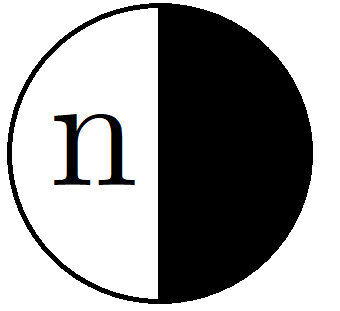
\includegraphics[width=3cm]{Immagini/neuronAutomata.png}}
	\hspace{5mm}
	\subfigure[Connections between neurons. The first is excitatory, the second is inhibitory]
	{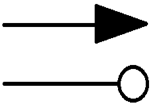
\includegraphics[width=3cm]{Immagini/linkAutomata.png}}
	\caption{Basic components of a neural network in the form of automata}
	\label{fig: elementiFondamentali}
\end{figure}


As in the previous articles, Minsky adheres to the classical model where the only delay in the network is an internal delay within neurons between receiving input and producing output. For completeness, we note that this choice differs from other models \cite{Burks1957}\cite{Copi1958}, where components dedicated to generating delay are proposed.\\
The remainder of the first part is dedicated to presenting various types of automata. We highlight a couple of particularly interesting ones:

\begin{itemize}
	\item Memory component: This allows us to remember that a certain cell was active in the previous state. To achieve this, we simply use a feedback loop, as shown in \autoref{fig:memory}.


\begin{figure}[!t]
	\centering
	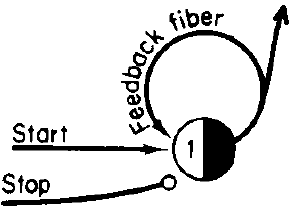
\includegraphics[width=4cm]{Immagini/memory.png}
	\caption{Memory component}
	\label{fig:memory}
\end{figure}



When the neuron receives the start signal, since its threshold is 1, it transitions from a resting state to an excited state. Being excited, it sends a signal to the rest of the network and also to itself. In the subsequent time steps, the neuron will remain excited, continuing to send signals through the feedback loop$\ldots$ Therefore, in the following time steps, the neuron will remain excited until it receives the inhibitory stop impulse.\\
Note that feedback loops give rise to cycles. As mentioned in the article by McCulloch and Pitts, this enhances expressiveness and prevents the neural network from "turning off" after propagating a signal.
\item Counter component: It is easy to understand that if we were able to "count," we could perform much more complex operations. We show two examples of counters in \autoref{fig: contatori}.

\begin{figure}[!t]
	\centering
	\subfigure[Counter capable of counting up to 2, also known as \emph{2 Scaler}]
	{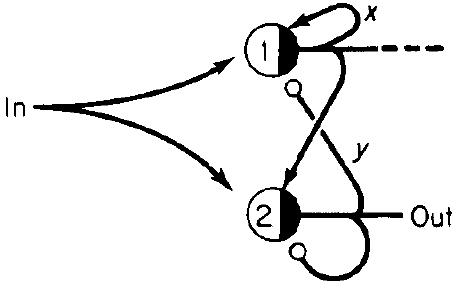
\includegraphics[width=5cm]{Immagini/counter2.png}}
	\hspace{5mm}
	\subfigure[By connecting \emph{k} components of 2 Scalers, we can count up to $2^k$]
	{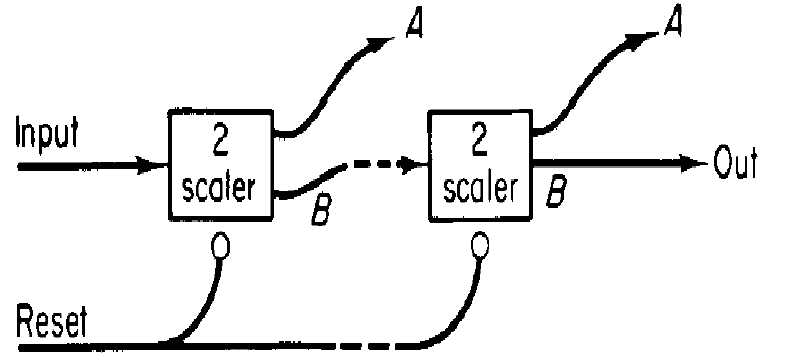
\includegraphics[width=6cm]{Immagini/counter2^k.png}}
	\caption{Counter components}
	\label{fig: contatori}
\end{figure}

The first one is a simple counter capable of counting up to two. By initially exciting the top neuron with an input, it remains excited thereafter due to the feedback loop $x$. Upon receiving a second signal, the bottom neuron also transitions from its quiescent state and produces an output to indicate that we have effectively counted up to two. Additionally, when the bottom neuron is excited, it sends a signal to inhibit both neurons, resetting the network to its initial state.\\
Suppose we encapsulate the described component and use it in series $k$ times as shown on the right side of \autoref{fig: contatori}, we achieve a counter capable of counting up to $2^k$.
\end{itemize}



The second part of the article introduces some theoretical elements and revisits the studies of Mealy and Moore to demonstrate the following theorem:

\begin{thm}
	Every finite state automaton is equivalent to, and can be simulated by, some neural network.
\end{thm}

At this point, Minsky proceeds to study some issues regarding the expressiveness of automata, aiming to identify a minimal set of components capable of representing every neural network. This set is referred to as the \emph{universal basis}.\\
Initially, the author attempts to construct a universal basis using only AND and OR nerve cells\footnote{The structure of such nerve cells is quite intuitive: an AND nerve cell receives two or more excitatory signals, and its excitation threshold is always equal to the number of signals it receives. An OR nerve cell receives two or more excitatory signals, and its excitation threshold is always one.}.\\
Unfortunately, these components are not sufficient, and to understand why, we must consider the issue of \emph{monotonicity}. A component is said to be \emph{monotonic} if it is not possible to decrease the output size by increasing the input size.\\
Both the AND and OR components are monotonic. This is easily understood: consider a network $R$ with a certain number of inputs and outputs. By replicating it and adding an excitatory signal, the number of output signals must be at least equal to the number of output signals from $R$.\\
It is easy to understand that to obtain a non-monotonic network, it is necessary to use inhibitory signals as well. There are some components called \emph{non-monotonic} that can decrease the output size while increasing the input size, all of which make use of inhibitory signals. Examples of non-monotonic components are shown in \autoref{fig:componentiInibitorie}. The last non-monotonic component is particularly important as it constitutes a universal basis on its own.\\

\begin{figure}[!t]
	\centering
	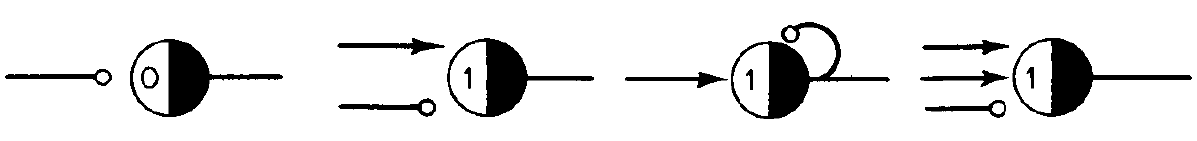
\includegraphics[width=12cm]{Immagini/componentiInibitorie.png}
	\caption{Non-monotonic components}
	\label{fig:componentiInibitorie}
\end{figure}


\vspace*{0.5cm}
To conclude, we also consider the historical context in which Minsky's article was written. Certainly, Kleene's research discussed in Chapter \ref{ch: Kleene} may have influenced his work, but we believe that the greater influence came from other studies.\\
An author frequently cited by Minsky in the article is John von Neumann. We believe that the development of automata capable of performing complex operations such as arithmetic derives from von Neumann's machine model. Moreover, as discussed in Chapter \ref{ch: origins}, there is a strong connection between von Neumann's model and neural networks. Given the close relationship between neural networks and automata, we believe that Minsky's work may have been influenced by von Neumann's studies.\\
Furthermore, when Minsky moved to the Massachusetts Institute of Technology in 1958, we believe he was guided in writing the article by the aforementioned studies of Mealy \cite{Mealy1955} and particularly those of Moore \cite{Moore1956}.\\
Between Moore's research in 1956 and the publication of Minsky's article in 1967, automata theory had time to spread and influence the studies of many, including Minsky.


\section{Conclusions}
In the preceding pages, we have traced the origins of neural networks. We examined the model of McCulloch and Pitts and how the concept of neurons influenced various fields of computer science seemingly unrelated to neural networks: computability theory, automata theory, and computing systems.\\
Next, we explored Kleene's studies and their theoretical contributions combined with the valuable invention of regular expressions.\\
Finally, we studied the work of Minsky, who made a significant contribution to the representation of neural networks.\\
At this point, considering the influence of the McCulloch and Pitts model on von Neumann's studies, it would be interesting to consider what direction computer science would have taken without their work.\\
Nevertheless, we can assert that the history of neural networks has brought with it a surprising amount of new ideas and concepts, playing a



\newpage

\begin{thebibliography}{3}
	\bibitem{McCulloch1943} Warren S. McCulloch e Walter Pitts \textit{A Logical Calculus of Ideas Immanent in Nervous Activity}, Bulletin of Mathematical Biophysics, volume 5, 1943.
	\bibitem{Carnap1937} Carnap Rudolf \textit{The Logical Syntax of Language}, Open Court Publishing, 1937.
	\bibitem{Russell1925} Bertrand Russell e Alfred N. Whitehead \textit{Principia Mathematica}, Cambridge University Press, 1925.
	\bibitem{Mealy1955} George H. Mealy \textit{A Method for Synthesizing Sequential Circuits}, Bell System Technical Journal: 1045–1079, 1955.
	\bibitem{Moore1956} Edward F. Moore \textit{Gedanken-experiments on Sequential Machines}, Automata Studies, Annals of Math, Princeton University Press: 129–153, 1956
	\bibitem{VonNeumann1945} John von Neumann \textit{First Draft of a Report on the EDVAC}, 1945
	\bibitem{Rashevsky1967} Nicolas Rashevsky \textit{Organismic Sets and Biological Epimorphism}, Bulletin of Mathematical Biophysics, volume 29, 1967.
	\bibitem{Kleene1956} Stephen C. Kleene \textit{Representation of events in nerve nets and finite automata}, Princeton University Press, 1956.
	\bibitem{Kleene1952} Stephen C. Kleene \textit{Introduction to metamathematics}, North Holland Publishing Co. , 1952.
	\bibitem{Minsky1967} Marvin L. Minsky \textit{Computation: Finite and Infinite Machines}: 32-66, Prentice Hall, 1967.
	\bibitem{Burks1957} Arthur W. Burks e Hao Wang \textit{The Logic of automata} JACM 4: 193-218 e 279-297, 1957.
	\bibitem{Copi1958} Irving M. Copi, Calvin C. Elgot e Jesse B. Wright \textit{Realization of events by logical nets}, JACM 5, num. 2: 181-196, 1958.
	\end{thebibliography}
\end{document}

McCulloch & Pitts: 1943
Kleene: 1956
Minksy: 1967
